\section{Diseño}
A continuación se presentan y explican algunas de las desiciones de diseño elegidas durante el desarrollo del trabajo practico.
Se decidió dividir la presentación en subsecciones para facilitar la comprensión de la misma, haciendo especial enfasis en aquellas que sentiamos eran de importancia para la comprensión del mismo.

Vale mencionar que si bien es cierto que se genero una idea general en el grupo antes de comenzar a reflejar las decisiones tomadas en codigo, el diseño en profundidad se termino de desarrollar y afinar en paralelo, mientras surgian cuestiones mismas relacionadas al propio desarrollo que no habian sido tenidos en cuenta en papel. 

\subsection{Acciones}
Entre las decisiones de diseño que consideramos de mayor relevancia, se encuentra el modelado de las jugadas como una sucesion de acciones que ocurren hasta que la pelota se vaya fuera del campo de juego. A su vez, modelados cada una de las distintas posibilidades de accion mediante una jerarquia. El mayor beneficio de esta decision es el de poder modificar los umbrales de exito de cada una de las acciones de manera sencilla y global para cualquier jugada, afectando lo minimo indispensable al resto del modelo del sistema.
\begin{center}

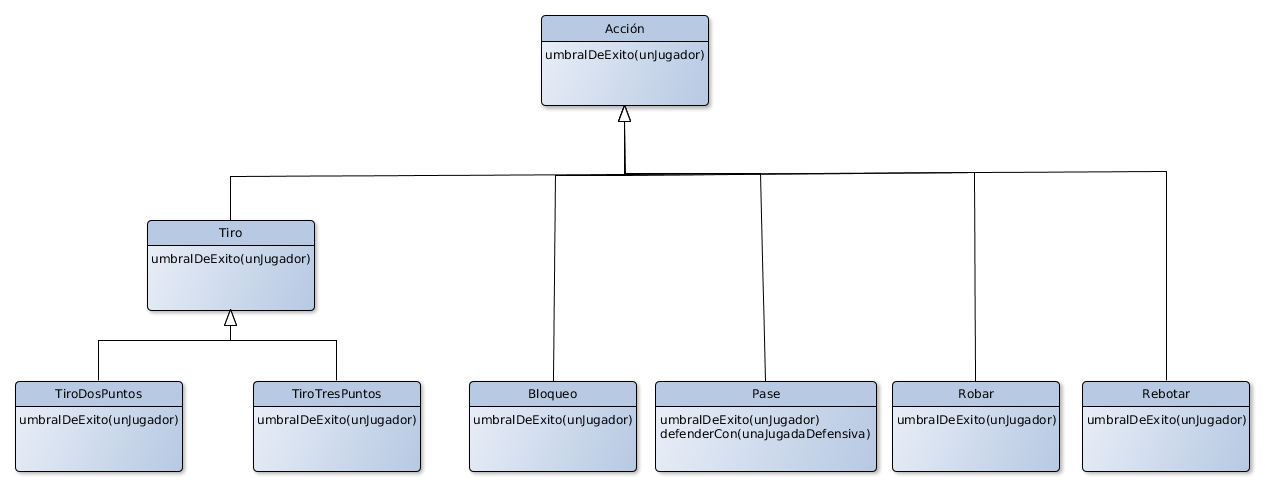
\includegraphics[scale=0.35]{diagramas/acciones.png}
\end{center}

\subsection{Jugadas}
Como dijimos anteriormente, se decidio modelar a las jugadas como una lista de acciones a ser ejecutadas. Es por esto que el concepto abstracto de jugada requiere poder conocer su lista de acciones y su proxima accion a ejecutar. Una vez mas, esta jerarquizacion, a demas de dejarnos representar el dominio de nuestro problema de forma correcta (MVP, ColectivaExterna, ColectivaInterna no son mas que distintas versiones de la idea de jugada)
\begin{center}
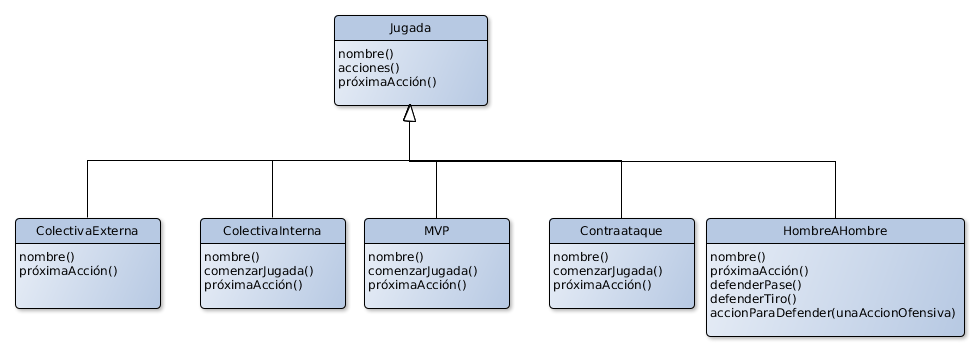
\includegraphics[scale=0.4]{diagramas/jugadas.png}
\end{center}


\subsection{DataManager}
Esta es, quizas, la decision mas conflictiva que tuvo el diseño planteado. Mientras una mitad del grupo sostenia que las distintas acciones que componen al DataManager presentado debian estar separadas en distintas clases, la otra se posicionaba firme en la idea de concentrar todo dentro de un 'Manager' simplificando el diseño de una forma que no impactaba en detrimento de la calidad.
Debido a un problema de tiempo del grupo, la opcion 'simplificadora' terminó ganando impulso y se impuso.
Esta clase reprensenta entonces todo el manejo de informacion que se realiza por fuera del juego propiamente dicho (actualizar jugadores, tecnicos, etc). En particular nosotros jerarquizamos esta idea abstracta con una clase de manejo de datos por archivos (FileDataManager) porque es la que usamos para nuestra implementacion, pero gracias a esta jerarquia nada impederia poder extender el diseño con, por ejemplo, un DBDataManager que implemente la carga de la informacion mediante una base de datos.

\begin{center}
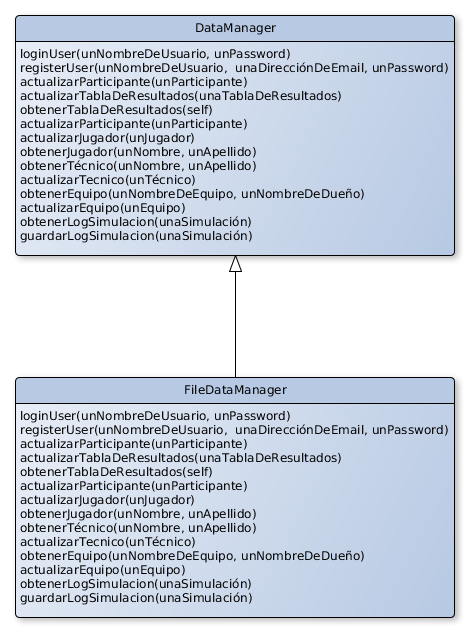
\includegraphics[scale=0.4]{diagramas/data_manager.png} 
\end{center}

\subsection{Nuevo tecnico}
A continuación, se ofrece el caso particular del alta de un nuevo tecnico, no porque sea una accion que consideremos relevante, sino como una forma de introducir el contexto en el que nuestro diseño se compone con el 'exterior'. Planteamos entonces una jerarquizacion entre los usuarios, dando la posibilidad a estos de ser tanto participantes del juego como administradores del mismo. Ademas se provee de un grupo de interfaces encargadas de 'representar' el accionar de cada uno de los formularios. Por consiguiente, la implementacion de las distintas interfaces por los formularios, permiten modelar el comportamiento correcto e integrarlo al resto del diseño sin mayores problemas.

\begin{center}
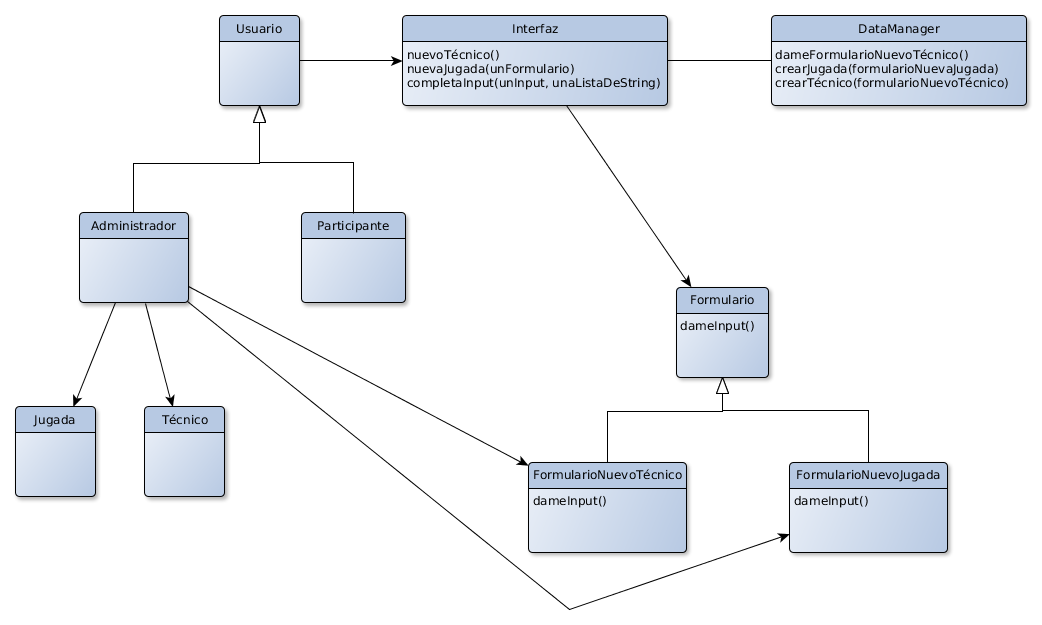
\includegraphics[scale=0.4]{diagramas/clases_nuevo_tecnico.png} 
\end{center}

\subsection{Secuencia de turnos}

\begin{center}
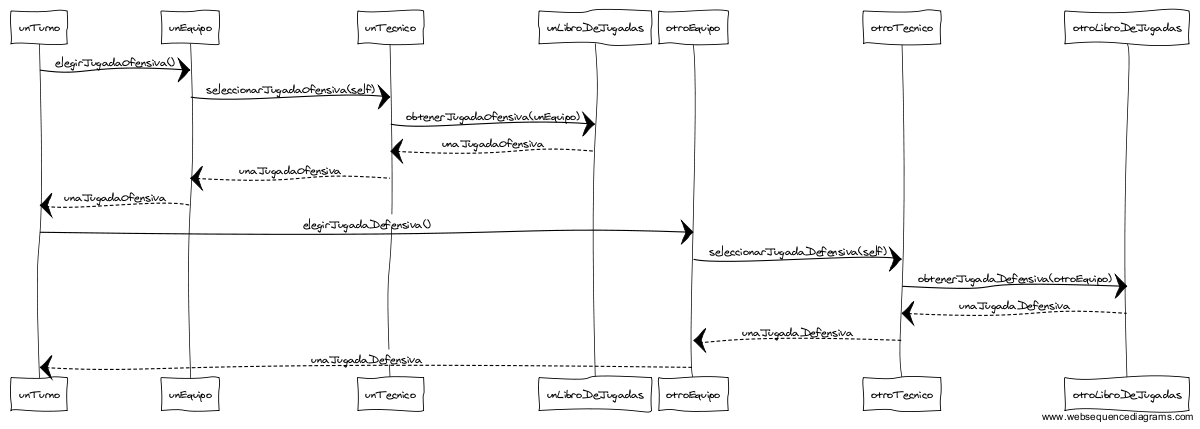
\includegraphics[scale=0.4]{diagramas/secuencias-turnos.png}
\end{center}


\begin{center}
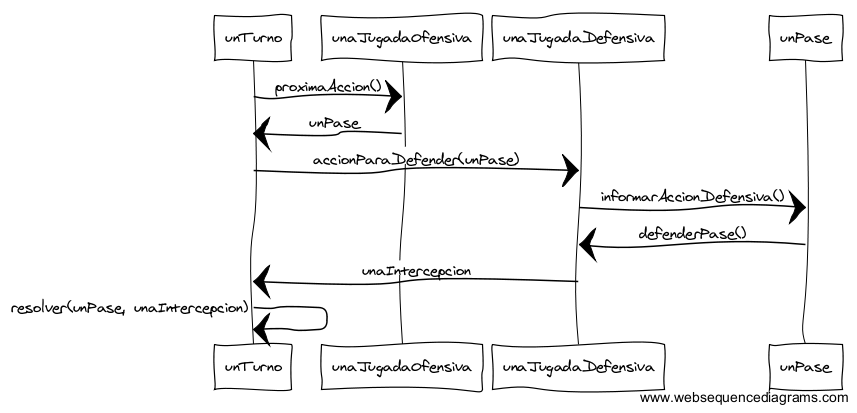
\includegraphics[scale=0.4]{diagramas/secuencia-turnos-1.png}
\end{center}


\subsection{Vision general}
El objetivo de este apartado es el de presentar un paneo general de la interrelacion de algunas de las clases mas importantes del diseño. Si bien algunas ya fueron mencionadas con anterioridad (jugadas, acciones, etc), decidimos repetirlas en pos de poder ofrecer una idea, a grandes rasgos, de su integracion dentro del sistema.

\begin{center}
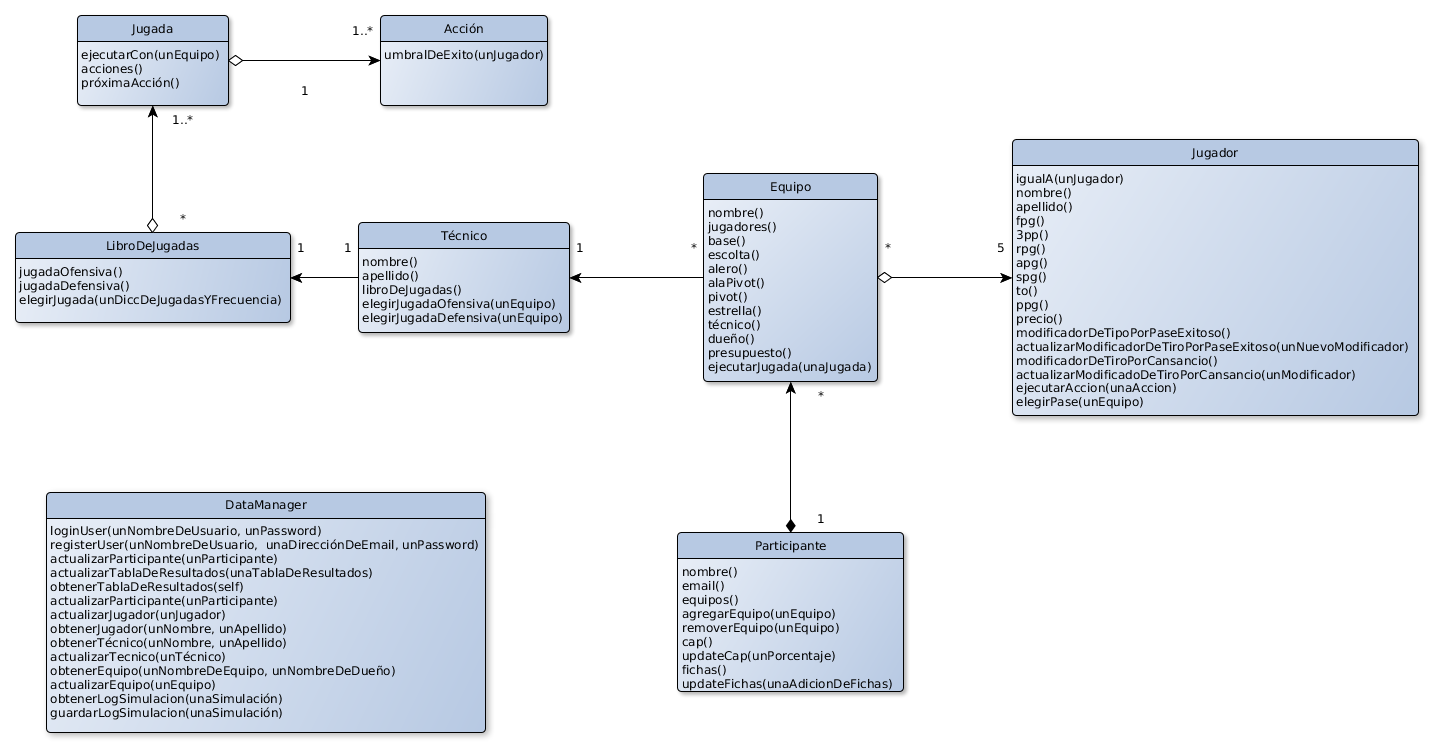
\includegraphics[scale=0.3]{diagramas/varias_clases.png}
\end{center}